%!TEX root = ../tesis.tex
\chapter{Soluci\'on Propuesta}
\label{sec:solucion}

Numerosas aplicaciones en el \'area del reconocimiento del habla han sido desarrolladas: \emph{Siri} \cite{AppleSiri}, \emph{Google Now} \cite{GoogleNow}, 
\emph{Dragon Naturally Speaking} \cite{DragonNaturallySpeaking}, etc. Cada una de estas
aplicaciones satisface distintos tipos de requerimientos establecidos por los usuarios finales. 

En el cap\'itulo anterior se presentó el desafío que supone el diseño de interfaces basadas 
en reconocimiento del habla, así como los requerimientos básicos de la aplicación a ser implementada como 
parte de este trabajo final de grado.

Este cap\'itulo presenta, justifica y eval\'ua la soluci\'on espec\'ifica al problema de implementar una interfaz
basada en reconomiento del habla para la aplicaci\'on escogida.


%!TEX root = ../tesis.tex

\section{Tecnolog\'ia a Utilizar}
\label{sec:tecnologia-utilizada}

Como se expone en la secci\'on~\ref{sec:problema-especifico}, se propone el dise\~no
de una interfaz para componer m\'usica utilizando la voz. Adem\'as, este trabajo 
opta por la metodolog\'ia de trabajo
de c\'odigo abierto, lo cual implica: 

\begin{itemize}
    \item Utilizar tecnolog\'ias de c\'odigo abierto para el desarrollo de la interfaz.
    \item Establecer un proceso de desarrollo transparente y abierto.
    \item Ofrecer la interfaz desarrollada, junto con su c\'odigo fuente, de manera libre 
        y gratuita para la comunidad de c\'odigo abierto.
\end{itemize}

La metodolog\'ia adoptada para implementar la interfaz permite utilizar un proyecto
existente como punto de partida, y as\'i dise\~nar e implementar una interfaz alternativa que permite
controlar la aplicaci\'on por comandos de voz. Adem\'as,
el hecho de incorporar una nueva interfaz, permite analizar
una de las motivaciones de la secci\'on~\ref{sec:motivacion}: un programa de composici\'on
musical, que recibe comandos sonoros y emite tambi\'en un resultado sonoro, podr\'ia ser
m\'as natural para el usuario. 

La interfaz desarrollada se denomina \emph{TamTam Listens} y se basa en tecnolog\'ias de c\'odigo abierto.
Toma como punto de partida la aplicaci\'on \emph{TamTam Edit} y para realizar el reconocimiento 
de comandos de voz utiliza los proyectos \emph{PocketSphinx} \cite{PocketSphinxHomePage} 
y \emph{Voxforge} \cite{Voxforge}.  A continuaci\'on se presentan los proyectos
utilizados como punto de partida para la soluci\'on implementada.

\subsection{TamTam Edit}
\label{sec:tamtam-edit}

La m\'usica es a menudo descrita como la forma m\'as pura de representaci\'on matem\'atica, es m\'as,
te\'oricos de la m\'usica han utilizado las matem\'aticas para resolver problemas musicales
\cite{TheSoundOfNumbers}. Esto sirvi\'o de inspiraci\'on para la creaci\'on del compendio de 
actividades\footnote{Una Actividad, es una aplicaci\'on en el entorno de escritorio \emph{Sugar}.}
conocido como \emph{TamTam} desarrollado para la computadora XO\footnote{La XO, es una computadora 
port\'atil de bajo costo y consumo desarrollada por el proyecto \gls{olpc}.},
con los siguientes objetivos:

\begin{itemize}
    \item Proveer a los ni\~nos un ambiente de informaci\'on cultural construyendo m\'usica y sonidos.
    \item Brindar una experiencia sonora/musical divertida para usuarios sin conocimientos musicales.
    \item Promover un camino hacia experiencias musicales m\'as sofisticadas.
    \item Promover un instrumento musical con su propio ``sonido''.
    \item Desarrollar un ambiente din\'amico y mutable que propone la simpleza y permite la complejidad.
    \item Favorecer la creaci\'on de m\'usica grupalmente.
    \item Introducir los conceptos musicales y otros como: programaci\'on y audio.
\end{itemize}

\emph{TamTam Edit} es una aplicaci\'on, que forma parte del conjunto de actividades musicales 
\emph{TamTam}, que proporciona una interfaz intuitiva para crear, modificar y organizar notas ubicadas 
en pistas virtuales.
Adem\'as incluye una paleta de casi cien tipos de sonidos y modelos de construcci\'on musical que permite 
crear distintos tipos de variaciones en estilos musicales \cite{TamTamWiki}.


Las secciones principales del programa se pueden observar en la figura~\ref{figure:ui-tamtam} 

\begin{figure}[H]
\centering
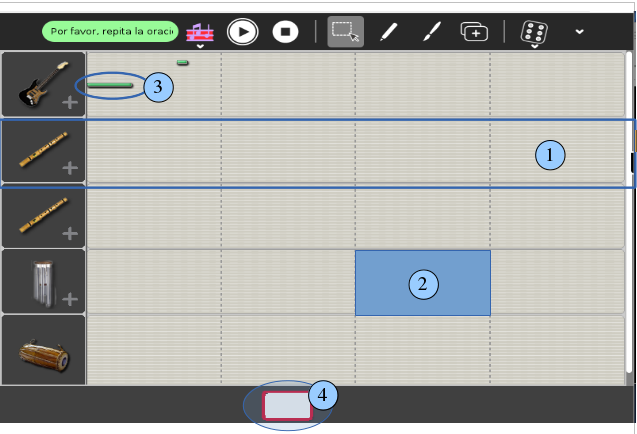
\includegraphics[width=0.8\textwidth]{./graphics/ui-tamtam-edit.png}
\caption{Interfaz de \emph{Tamtam Edit} y sus secciones principales}
\label{figure:ui-tamtam}
\end{figure}

Como se puede apreciar en la figura~\ref{figure:ui-tamtam}, la interfaz se encuentra organizada en 
cinco pistas y cada pista (1) tiene asociada un instrumento (la quinta pista esta reservada para
instrumentos de tipo bater{\'\i}a). Cada pista se divide en 4 
compases (del comp\'as uno al cuatro) y cada comp\'as (2) se divide en 12 tiempos (del uno al doce). 
Las notas (3) se dibujan en los compases, como se puede ver, la longitud de la nota indica su 
duraci\'on y su altura el tipo de nota. Adem\'as la aplicaci\'on esta organizada en partituras (4), que 
son como hojas de cuaderno, y son \'utiles para componer m\'usicas largas.

En general, la interacci\'on entre el usuario y \foreign{TamTam Edit} que se presenta en
la figura~\ref{figure:ui-tamtam} se realiza de modo tradicional.
El usuario utiliza el teclado y el rat\'on para interactuar con la aplicaci\'on a trav\'es de elementos
gr\'aficos como botones y men\'us. 

Este trabajo de grado busca incorporar un medio de interacci\'on alternativo al propuesto por \emph{TamTam Edit}. 
A continuaci\'on se presentan los motivos que determinaron la elecci\'on de esta aplicaci\'on como punto de partida:

\begin{itemize}
    \item Impacto social: \emph{TamTam Edit} es una aplicaci\'on que forma parte de la plataforma establecida
    por el proyecto \gls{olpc}, el cual busca potenciar el proceso educativo \cite{OLPC}. 
    Los ni\~nos con alg\'un tipo de discapacidad tienen a menudo problemas para utilizar una computadora mediante
    dispositivos perif\'ericos tradicionales como el mouse o el teclado.

    En estos casos, la posibilidad de operar esta actividad mediante la voz ser{\'\i}a de gran beneficio 
    para los ni\~nos, mejorando la accesibilidad de la plataforma, y generando por tanto un impacto social
    positivo importante.
    \item Naturalidad de interacci\'on: utilizar la voz para interactuar con una aplicaci\'on podr{\'\i}a
    ofrecer una mayor naturalidad con respecto al enfoque tradicional de interacci\'on, teniendo en cuenta
    que es el medio de interacci\'on entre las personas.
    \item No reinventar la rueda: como el objetivo es incorporar una interfaz basada en reconocimiento del
    habla a una aplicaci\'on, se elige \emph{TamTam Edit} para no construir la aplicaci\'on desde cero,
    sino extender las capacidades de una ya existente.
    \item C\'odigo abierto: el motivo anterior es posible gracias a que \emph{TamTam Edit} es un 
    proyecto de c\'odigo abierto, lo cual brinda a los desarrolladores la libertad de extender las 
    funcionalidades de la aplicaci\'on.
    \item Lenguaje de programaci\'on: la actividad se encuentra implementada en el lenguaje de 
    programaci\'on Python. La librer{\'\i}a de reconocimiento del habla a ser utilizada proporociona 
    \emph{bindings} 
    \footnote{Un \emph{binding} es un componente \emph{software}
   que permite hacer uso de las funcionalidades prove{\'\i}das por una librer{\'\i}a, implementada
    en un determinado lenguaje de programaci\'on, utilizando un lenguaje de programaci\'on diferente. 
    En este caso particular, \emph{Pocketsphinx} est\'a implementado en C y C++.} para 
    este lenguaje, lo cual supone una ventaja importante para la implementaci\'on de la interfaz.
\end{itemize}


\subsection{Voxforge}
\foreign{Voxforge} es un proyecto que busca recopilar grabaciones de voz de modo a crear 
y ofrecer varios corpus de habla bajo una licencia que permita su libre utilizaci\'on. 

A partir de estos corpus, es posible construir modelos ac\'usticos para su uso con motores de 
reconocimiento del habla de c\'odigo abierto, como \foreign{Pocketsphinx}.

\foreign{Voxforge} cuenta con grabaciones en diferentes idiomas, entre ellos ingĺ\'es, franc\'es, 
alem\'an y espa\~nol.


\subsection{PocketSphinx}

El cap\'itulo~\ref{sec:tecnologias} clasifica a las herramientas que permiten implementar soluciones
basadas en reconocimiento del habla en tres categor\'ias: Aplicaciones, \gls{api}s y Librer\'ias. 
Dada la naturaleza de este trabajo, se opta por elegir una librer\'ia para implementar la interfaz
alternativa a la ofrecida por \emph{TamTam Edit}.

Para la implementaci\'on de la interfaz operable a trav\'es de la voz se elige la librer\'ia 
\emph{PocketSphinx} que, como se menciona en la secci\'on~\ref{sec:pocketsphinx}, es un motor de 
reconocimiento del habla orientado a la optimizaci\'on del rendimiento y la portabilidad.

Uno de los objetivos espec\'ificos de este trabajo es aplicar y contrastar en la pr\'actica
los conocimientos te\'oricos adquiridos. Como indica la secci\'on~\ref{sec:librerias}, una librer\'ia es
el tipo de herramienta que requiere un conocimiento t\'ecnico espec\'ifico del \'area, adem\'as de
brindar una alta flexibilidad permitiendo al programador manipular los distintos componentes del
proceso de reconocimiento del habla. Por este motivo, una librer\'ia se considera la herramienta 
m\'as adecuada para cumplir el objetivo mencionado anteriormente.

A continuaci\'on se presentan los motivos t\'ecnicos que determinaron la elecci\'on de esta librer\'ia:

\begin{itemize}
    \item \emph{PocketSphinx} est\'a orientada a la optimizaci\'on del rendimiento, resultando adecuada 
    para sistemas con recursos limitados, como la computadora \emph{XO}.
    \item La librer\'ia es un proyecto de c\'odigo abierto, por lo tanto se cumple la metodolog\'ia 
    de trabajo adoptada.
    \item \emph{PocketSphinx} ofrece soporte \emph{offline}, lo cual permite su utilizaci\'on en ambientes
    sin conexi\'on a internet, como ocurre frecuentemente con las \emph{XO}.
    \item Existen \foreign{bindings} para el lenguaje de programaci\'on Python, lo cual hace muy 
    sencilla la tarea de utilizar la librer\'ia desde el c\'odigo Python.
\end{itemize}

\foreign{PocketSphinx} implementa el proceso del reconocimiento del habla basado en el enfoque 
estad{\'\i}stico, el cual se present\'o en el cap{\'\i}tulo~\ref{sec:proceso}. La librer{\'\i}a incluye
los diferentes algoritmos necesarios para las fases del proceso.

\begin{figure}[H] 
\centering
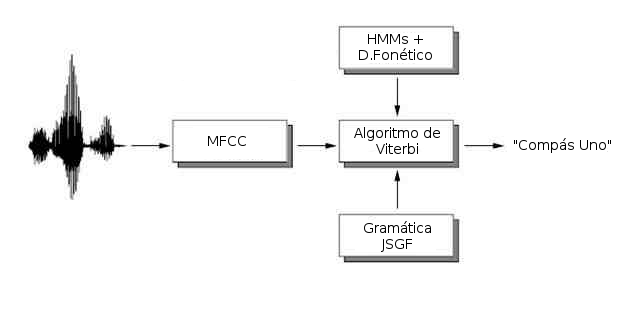
\includegraphics[width=0.8\textwidth]{./graphics/pocketsphinx.png}
\caption{Reconocimiento del habla mediante PocketSphinx. Gr\'afico basado en \cite{VerenichASR}.}
\label{figure:proceso-pocketsphinx}
\end{figure}

Como conjunto de caracter{\'\i}sticas espectrales, \foreign{Pocketsphinx} utiliza los coeficientes
espectrales en las frecuencias de mel (MFCC por sus siglas en ingl\'es).

En los \gls{hmm} del modelo ac\'ustico, utiliza mezclas Gaussianas para definir las probabilidades de 
transici\'on entre estados. El diccionario fon\'etico debe ser definido por el desarrollador.

Aunque \foreign{PocketSphinx} soporta modelos de lenguaje basados en n-gramas, para este trabajo 
se utiliza un modelo de lenguaje basado en gram\'atica. Esto se debe a la simpleza del lenguaje y a la 
falta de datos de entrenamiento para un modelo estad{\'\i}stico del mismo.

Como decodificador se utiliza el algoritmo de Viterbi, haciendo uso de la t\'ecnica de b\'usqueda en haz
para reducir el espacio de b\'usqueda.

\section{Tamtam Listens}
\label{sec:tamtam-listens}

La aplicación desarrollada, denominada \emph{Tamtam Listens}, es el resultado de la combinación
de las tecnolog\'ias mencionadas anteriormente. Por lo tanto, \emph{Tamtam Listens} representa una
interfaz de interacci\'on alternativa para la aplicaci\'on \emph{Tamtam Edit}.

El reconocimiento de los comandos de voz se implement\'o como un servicio de \emph{dbus}\cite{Dbus2013}, que es
un mecanismo para comunicaci\'on entre procesos de linux. Por lo tanto, el servicio puede ser utilizado
no solo por \emph{Tamtam Listens} si no por cualquier aplicaci\'on de linux. 

\emph{Pocketsphinx} requiere de un modelo ac\'ustico y un modelo de lenguaje para realizar
el reconocimiento de comandos. Para el modelo ac\'ustico se utiliz\'o el prove\'ido por el proyecto \emph{Voxforge}
\cite{Voxforge}, que es un proyecto que busca proveer modelos ac\'usticos para motores de reconocimientos
de c\'odigo abierto. Para el modelo de lenguaje se defini\'o una gram\'atica en formato \gls{jsgf} 
\cite{JSGF2000}, que permiti\'o definir los comandos soportados por la aplicaci\'on de una manera sencilla. 

\subsection{Gram\'atica}

A continuaci\'on se puede observar un fragmento de la gram\'atica \gls{jsgf} utilizada para definir 
los comandos soportados por \emph{Tamtam Listens}, m\'as adelante se presentar\'an los comandos
en forma de grafo para una mejor comprensi\'on.

\lstset{
  basicstyle=\scriptsize,        % the size of the fonts that are used for the code
  breakatwhitespace=false,         % sets if automatic breaks should only happen at whitespace
  frame=single,                    % adds a frame around the code
  language=Octave,                 % the language of the code
  numbersep=5pt,                   % how far the line-numbers are from the code
  showstringspaces=false,          % underline spaces within strings only
  stepnumber=2,                    % the step between two line-numbers. If it's 1, each line will be numbered
  tabsize=2                       % sets default tabsize to 2 spaces
}

\begin{figure}[H]
\begin{lstlisting}
#JSGF V1.0;
grammar tamtam;

public <tamtam-listens> = <comando> | <pagina> | <pista-a>     | <pista-b>  | 
                          <seleccionar-compas> | <crear-nota>  | <seleccionar-nota> | 
                          <duplicar-nota>      | <borrar-nota> | <volumen> | <tempo> | 
                          <configurar-nota>    | <loop>;

<comando>  = REPRODUCIR MUSICA  | PAUSAR MUSICA   | PARAR MUSICA | GENERAR MUSICA | 
             CREAR NUEVA MUSICA | EXPORTAR MUSICA | SALIR DE TAMTAM;
<pagina>   = ( CREAR NUEVA | DUPLICAR | LIMPIAR ) PARTITURA | PARTITURA <orden>;
<orden>    = ( ANTERIOR | SIGUIENTE );
<loop>     = (BASURA)+;
\end{lstlisting}
\caption{Fragmento de la gram\'atica utilizada en \emph{Tamtam Listens}}
\end{figure}

Los comandos pueden clasificarse en Generales (G), de Pista (P) y de Comp\'as (C). A continuaci\'on
se presentan los distintos comandos soportados, utilizando grafos para representarlos y as\'i facilitar
su comprensi\'on. El nodo coloreado hace referencia a la \'ultima palabra de un comando v\'alido para la aplicaci\'on

\subsubsection{Comandos Generales}

\begin{figure}[H] 
\centering
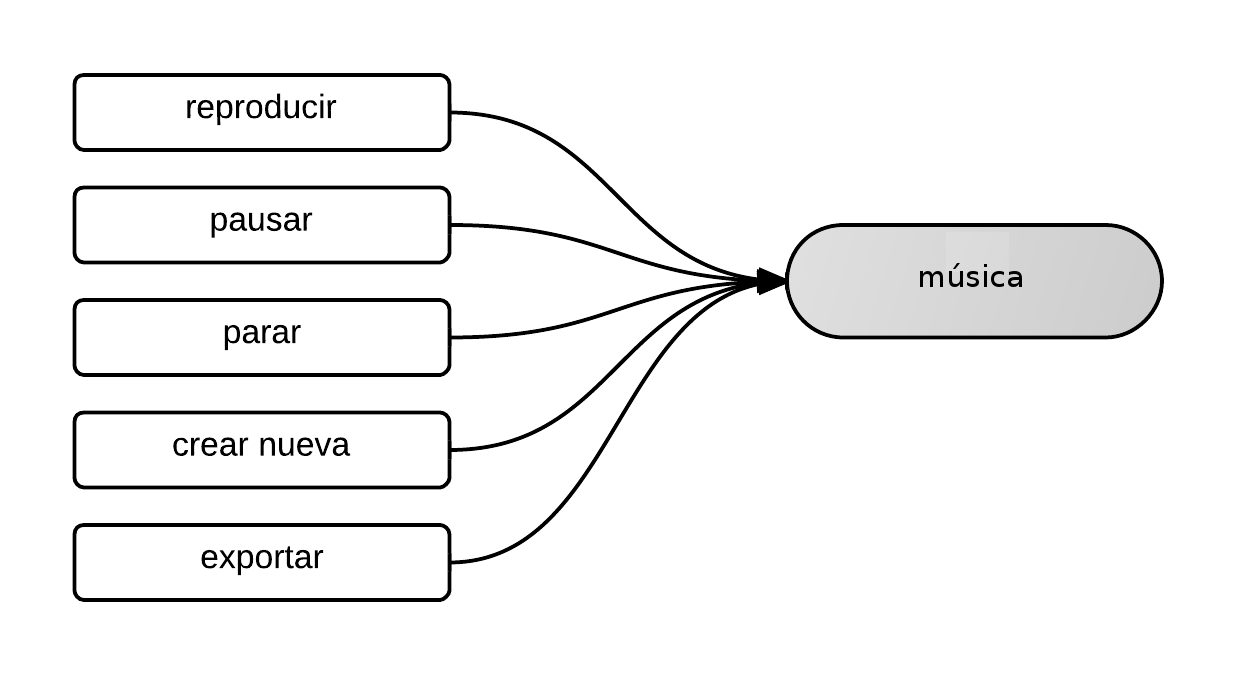
\includegraphics[width=0.5\textwidth]{./graphics/cmd-musica.png}
\caption{Comandos para reproducir, pausar, parar, exportar y crear una m\'usica}
\label{figure:cmd-crear-musica}
\end{figure}

\begin{figure}[ht]
\begin{minipage}[b]{0.5\linewidth}
\centering
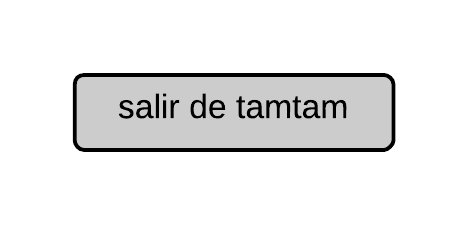
\includegraphics[width=0.6\linewidth]{./graphics/salir.png}
\caption{Comando para salir de la aplicaci\'on}
\label{figure:cmd-salir}
\end{minipage}
\quad
\begin{minipage}[b]{0.5\linewidth}
\centering
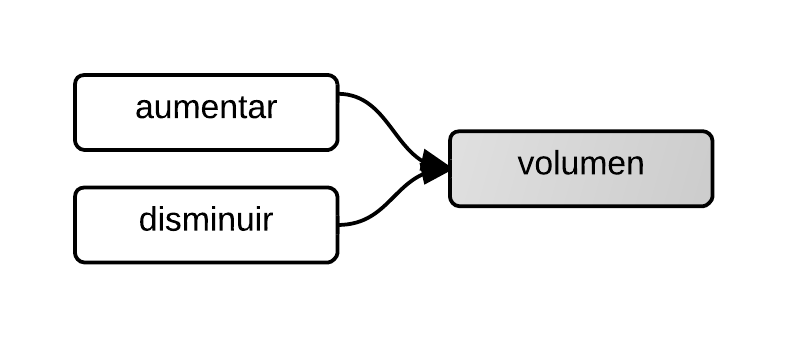
\includegraphics[width=0.6\linewidth]{./graphics/cmd-vol.png}
\caption{Comandos para aumentar/disminuir el volumen general}
\label{figure:cmd-vol}
\end{minipage}
\end{figure}


\begin{figure}[ht]
\begin{minipage}[b]{0.5\linewidth}
\centering
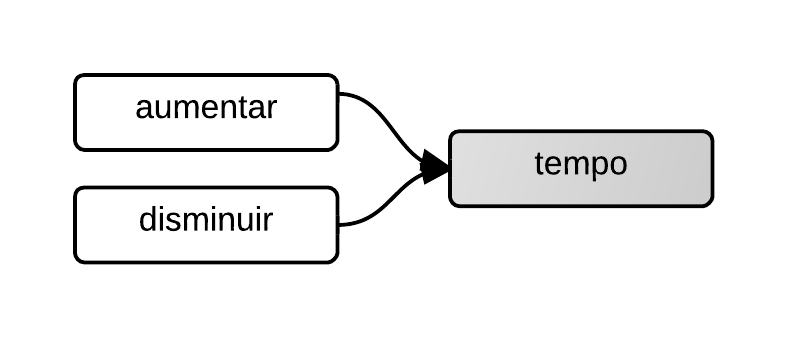
\includegraphics[width=0.6\linewidth]{./graphics/cmd-tempo.png}
\caption{Comandos para aumentar/disminuir el tempo general de al aplicaci\'on}
\label{figure:cmd-tempo}
\end{minipage}
\quad
\begin{minipage}[b]{0.5\linewidth}
\centering
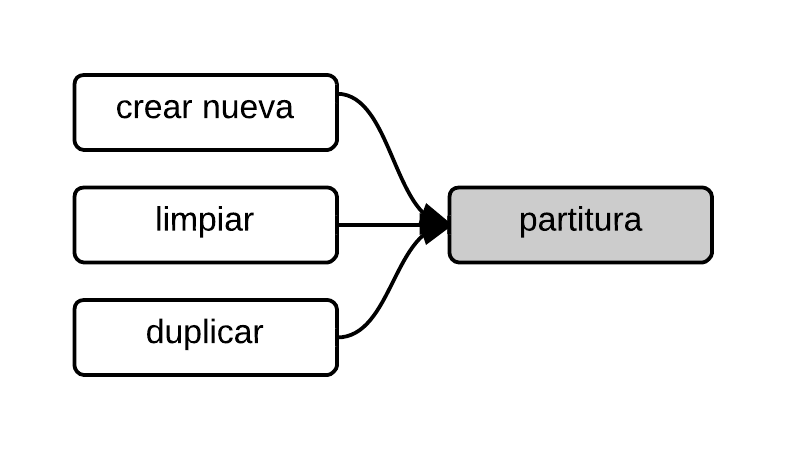
\includegraphics[width=0.6\linewidth]{./graphics/partitura-1.png}
\caption{Comandos para crear, limpiar y duplicar la partitura actual}
\label{figure:cmd-partitura-1}
\end{minipage}
\end{figure}


\begin{figure}[H]
\begin{minipage}[b]{0.5\linewidth}
\centering
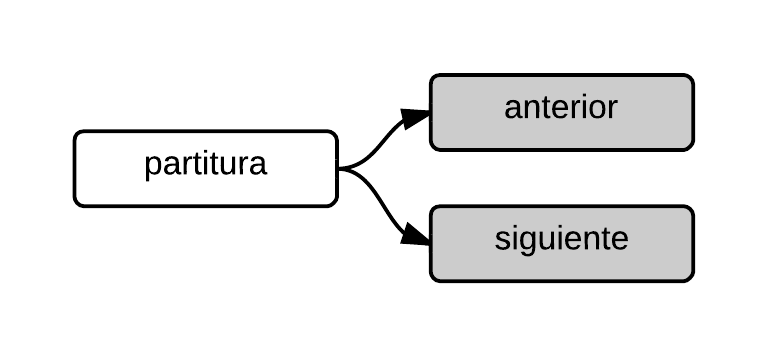
\includegraphics[width=0.6\linewidth]{./graphics/partitura-2.png}
\caption{Comandos para navegar entre partituras}
\label{figure:cmd-partitura-2}
\end{minipage}
\quad
\begin{minipage}[b]{0.5\linewidth}
\centering
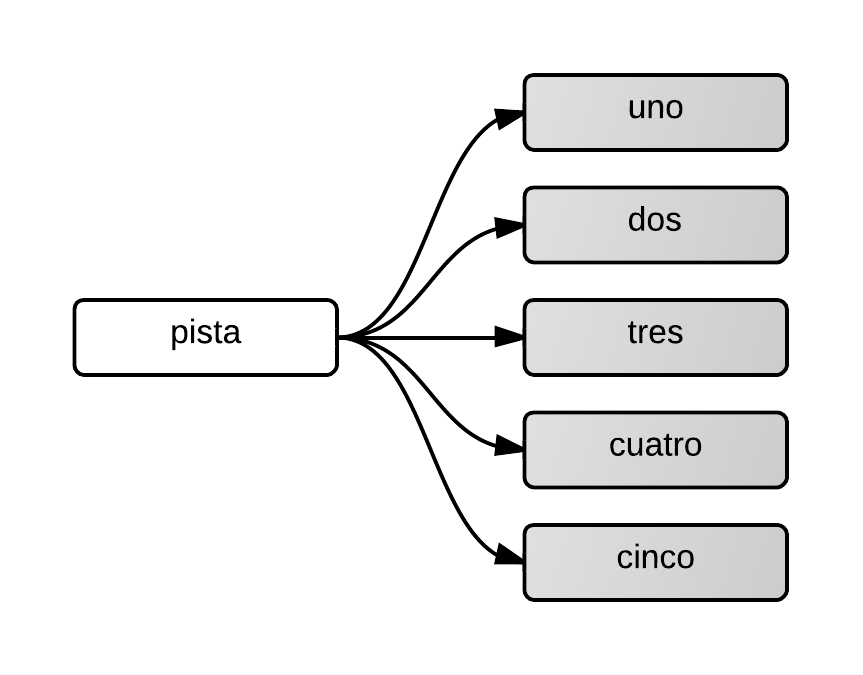
\includegraphics[width=0.6\linewidth]{./graphics/cmd-pista-1.png}
\caption{Comando para ubicarse en una pista}
\label{figure:cmd-partitura-1}
\end{minipage}
\end{figure}


\begin{figure}[H]
\begin{minipage}[b]{0.5\linewidth}
\centering
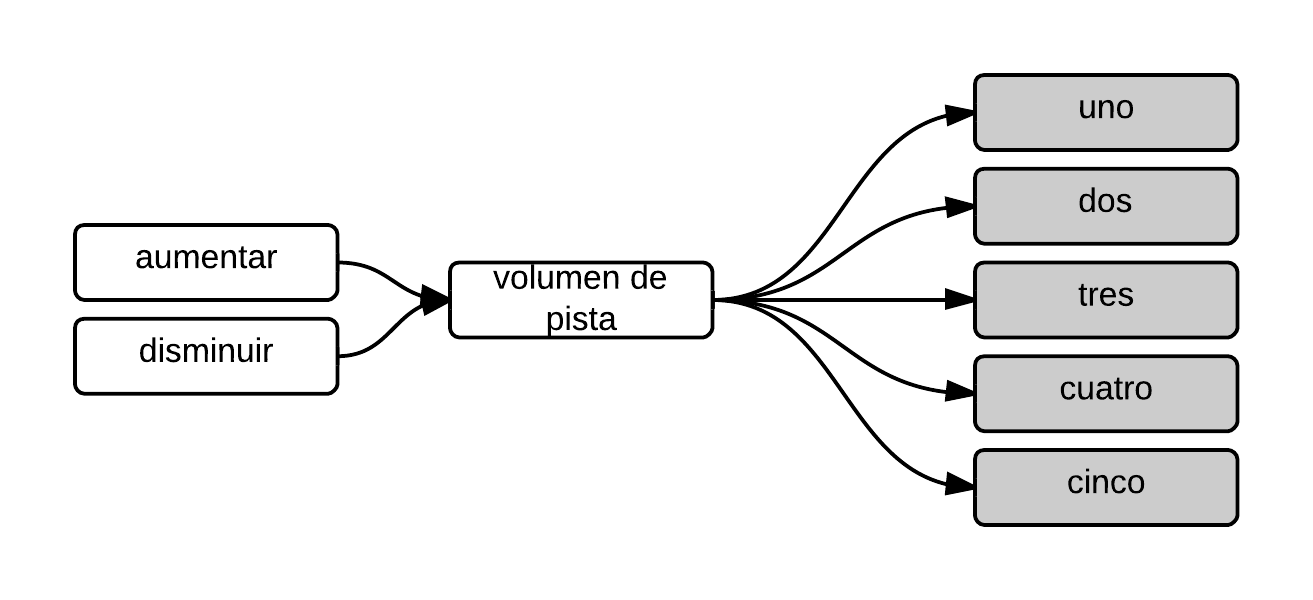
\includegraphics[width=0.8\linewidth]{./graphics/vol-pista.png}
\caption{Comandos para aumentar/disminuir el volumen de una pista en particular}
\label{figure:cmd-vol-pista}
\end{minipage}
\quad
\begin{minipage}[b]{0.5\linewidth}
\centering
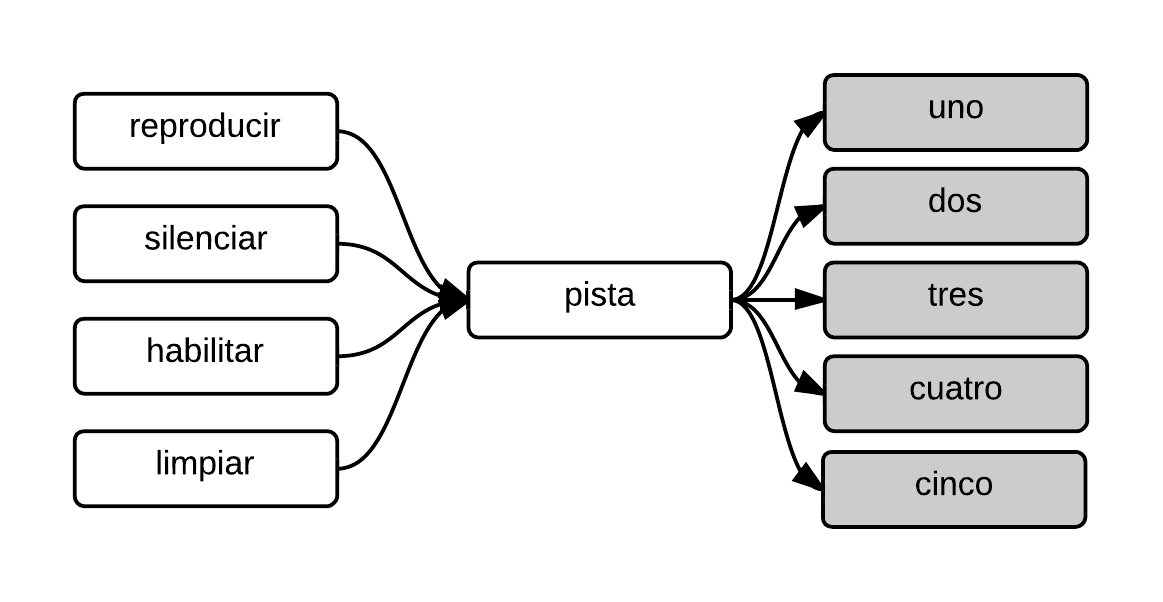
\includegraphics[width=0.9\linewidth]{./graphics/rep-pista.png}
\caption{Comandos para reproducir, silenciar, habilitar y limpiar una pista en particular}
\label{figure:cmd-rep-pista}
\end{minipage}
\end{figure}

\begin{figure}[H]
\centering
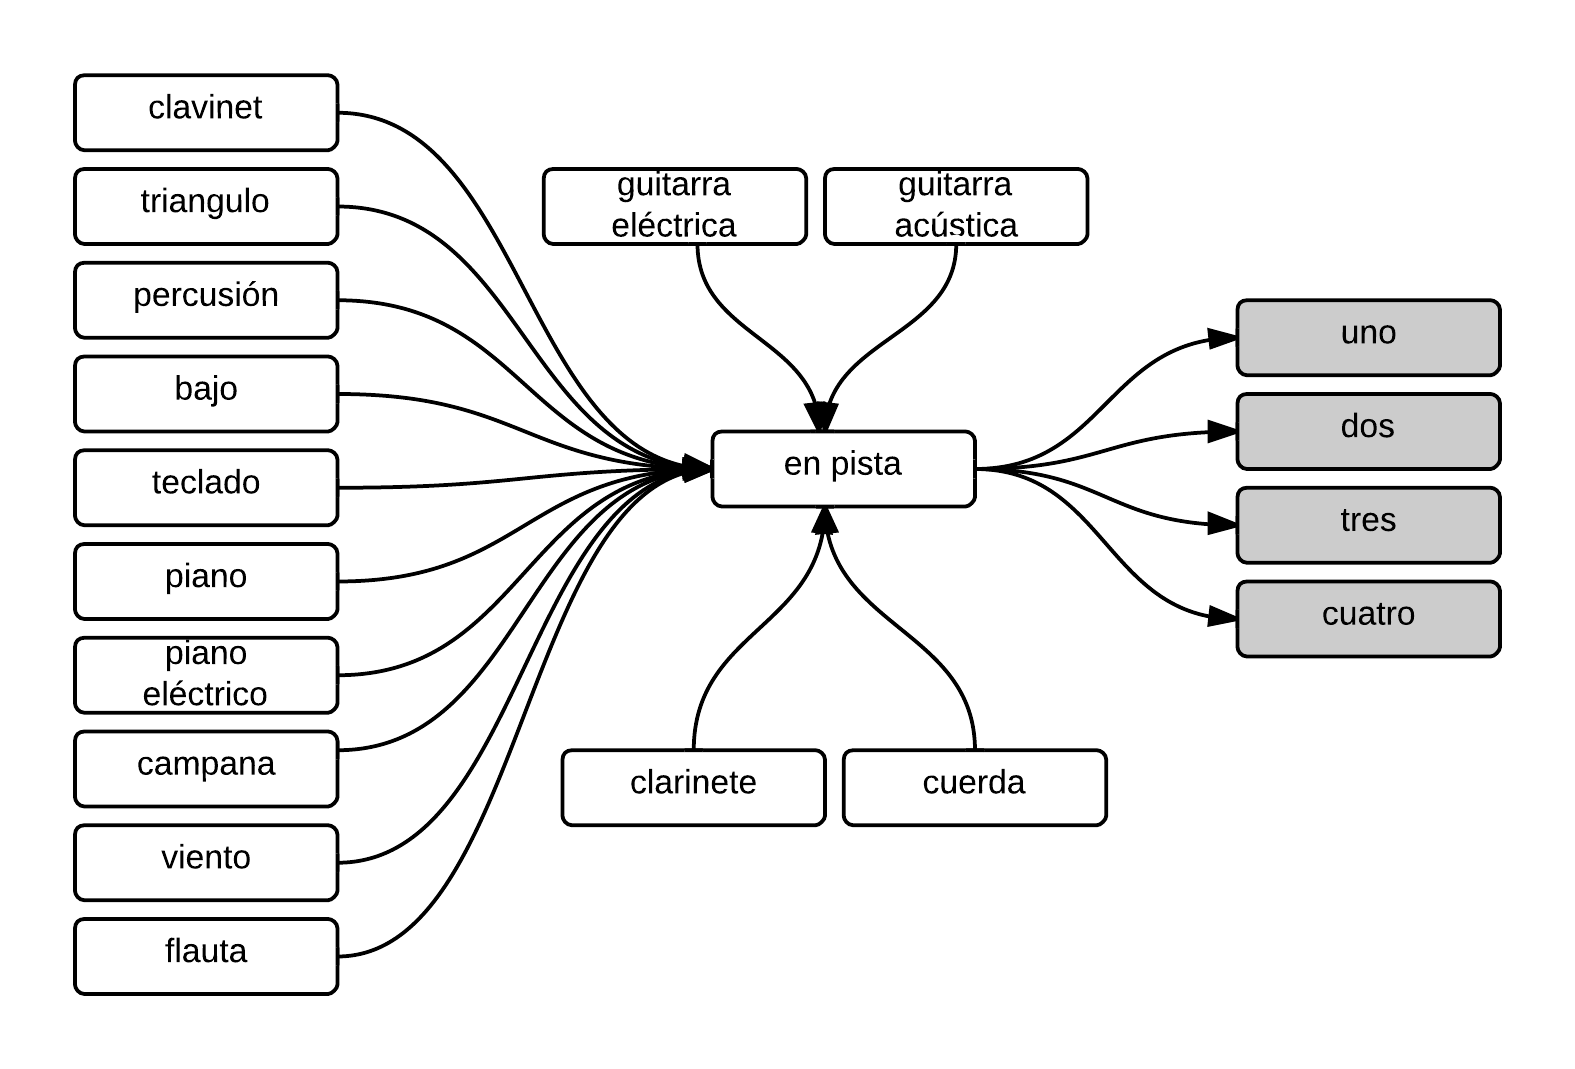
\includegraphics[width=0.8\textwidth]{./graphics/inst-p1-4.png}
\caption{Selecci\'on de instrumento para pistas del uno al cuatro}
\label{figure:cmd-inst-p1-4}
\end{figure}

\begin{figure}[H]
\begin{minipage}[b]{0.5\linewidth}
\centering
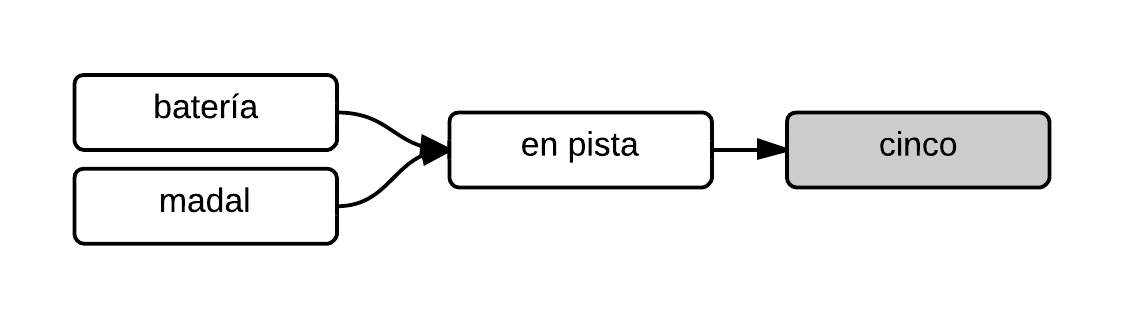
\includegraphics[width=1\linewidth]{./graphics/inst-p5.png}
\caption{Selecci\'on de instrumento para la pista cinco}
\label{figure:cmd-inst-p5}
\end{minipage}
\quad
\begin{minipage}[b]{0.5\linewidth}
\centering
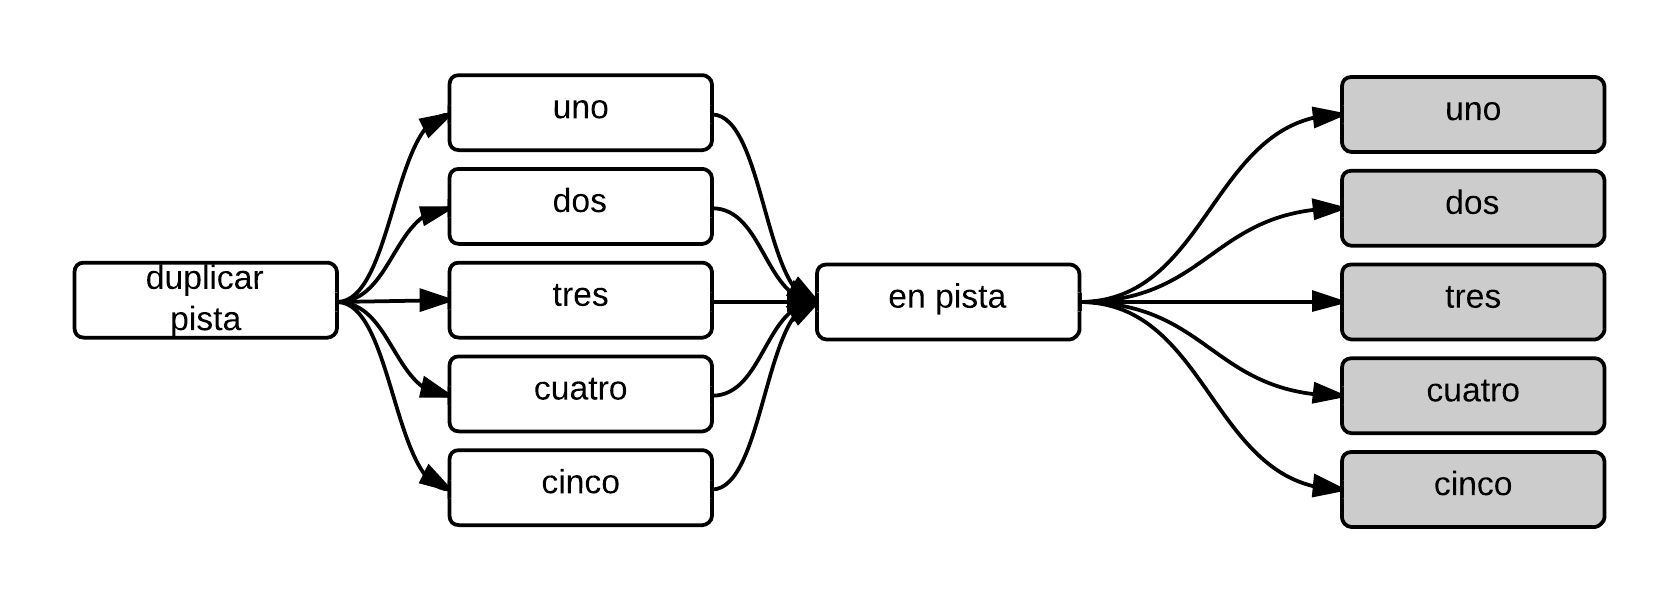
\includegraphics[width=1\linewidth]{./graphics/dup-pista.png}
\caption{Comando para duplicar las notas de una pista en otra}
\label{figure:cmd-dup-pista}
\end{minipage}
\end{figure}

\subsubsection{Comandos de Pista}

Este comando nos ubica dentro de una pista en particular. Por lo tanto, se debe
seleccionar una pista para poder utilizar este comando.

\begin{figure}[H]
\centering
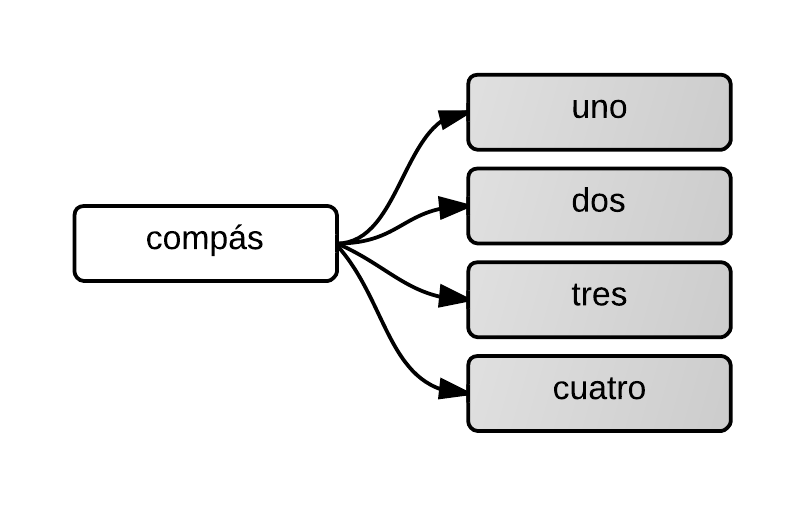
\includegraphics[width=0.4\linewidth]{./graphics/cmd-compas.png}
\caption{Comando para ubicarse en un comp\'as}
\label{figure:cmd-compas}
\quad
\end{figure}

\subsubsection{Comandos de Comp\'as}

Estos comandos son muy importantes para la aplicación ya que nos permiten crear, modificar, 
eliminar las notas musicales.

\begin{figure}[H]
\begin{minipage}[b]{0.5\linewidth}
\centering
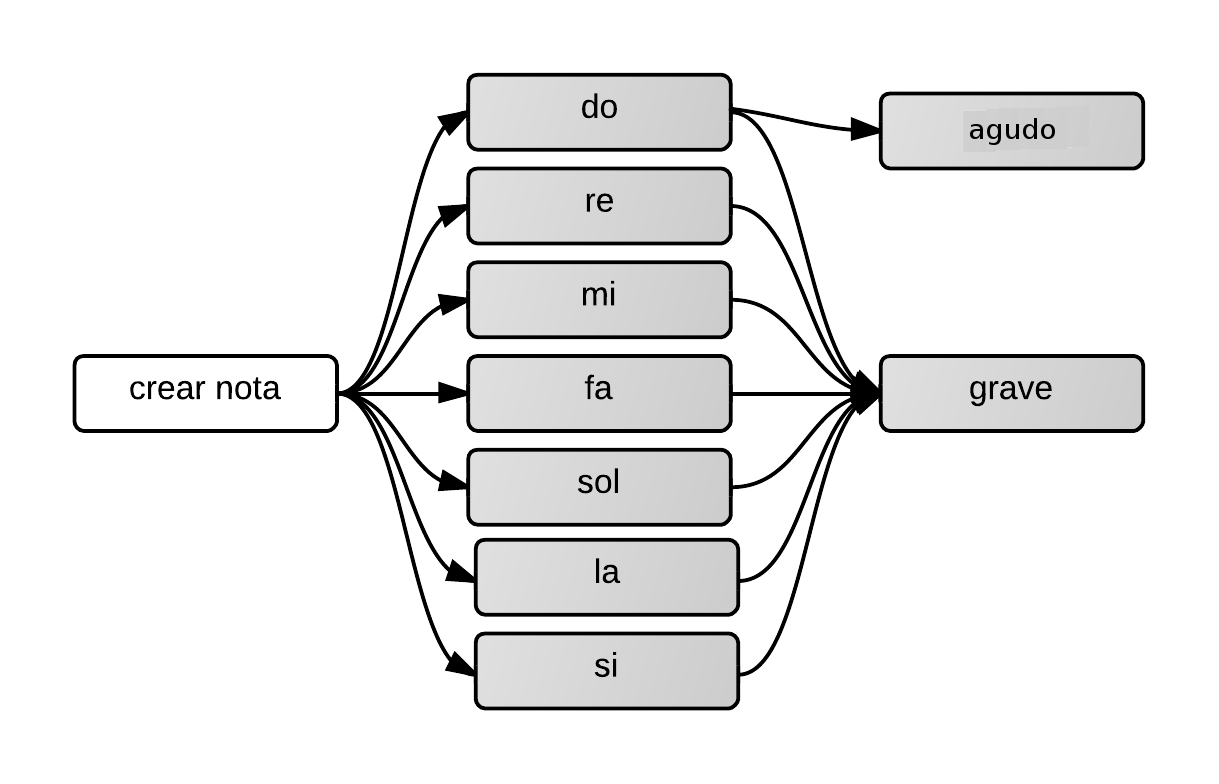
\includegraphics[width=1\linewidth]{./graphics/cmd-crear-nota.png}
\caption{Comando para crear una nota}
\label{figure:cmd-crear-nota}
\end{minipage}
\quad
\begin{minipage}[b]{0.5\linewidth}
\centering
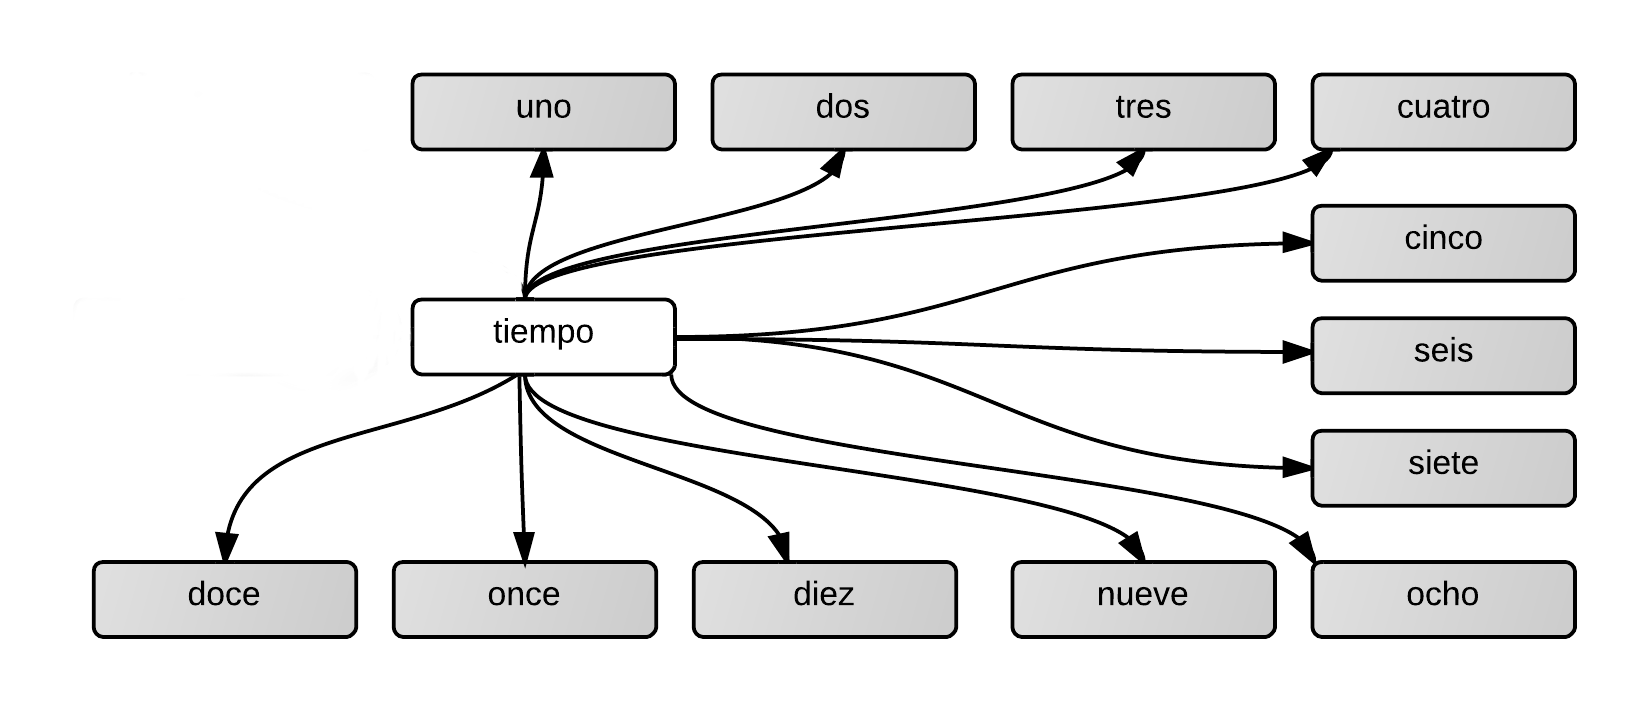
\includegraphics[width=1.1\linewidth]{./graphics/cmd-tiempo-compas.png}
\caption{Comando para ubicarse en un tiempo dado, dentro de un comp\'as}
\label{figure:cmd-tiempo-compas}
\end{minipage}
\end{figure}

\begin{figure}[H]
\begin{minipage}[b]{0.5\linewidth}
\centering
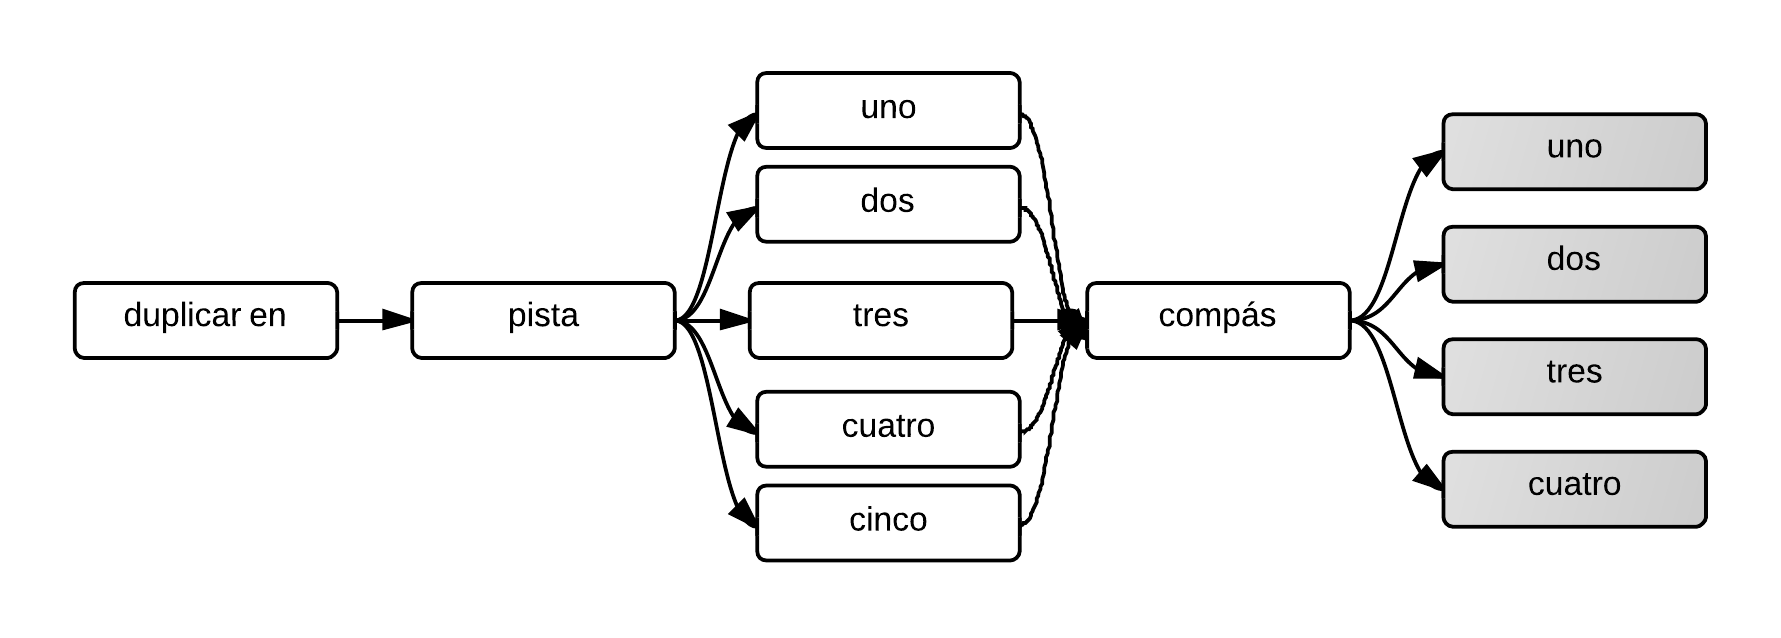
\includegraphics[width=1.2\linewidth]{./graphics/cmd-dup-nota.png}
\caption{Comando para duplicar una nota previamente seleccionada}
\label{figure:cmd-dup-nota}
\end{minipage}
\quad
\begin{minipage}[b]{0.5\linewidth}
\centering
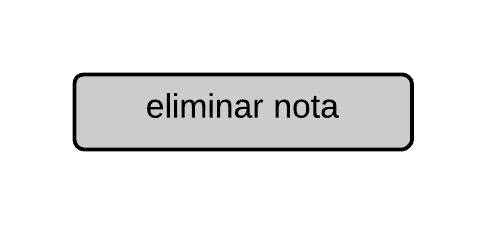
\includegraphics[width=0.5\linewidth]{./graphics/del-note.png}
\caption{Comando para eliminar un nota previamente seleccionada}
\label{figure:cmd-del-nota}
\end{minipage}
\end{figure}


\begin{figure}[H]
\begin{minipage}[b]{0.5\linewidth}
\centering
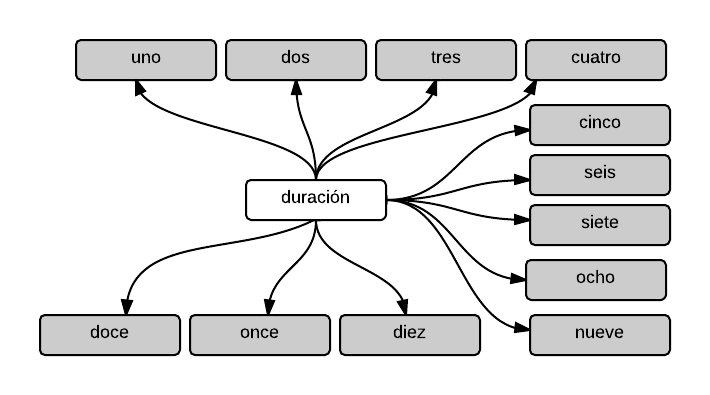
\includegraphics[width=0.9\linewidth]{./graphics/cmd-dur.png}
\caption{Comando que permite configurar la duraci\'on de una nota}
\label{figure:cmd-dur}
\end{minipage}
\quad
\begin{minipage}[b]{0.5\linewidth}
\centering
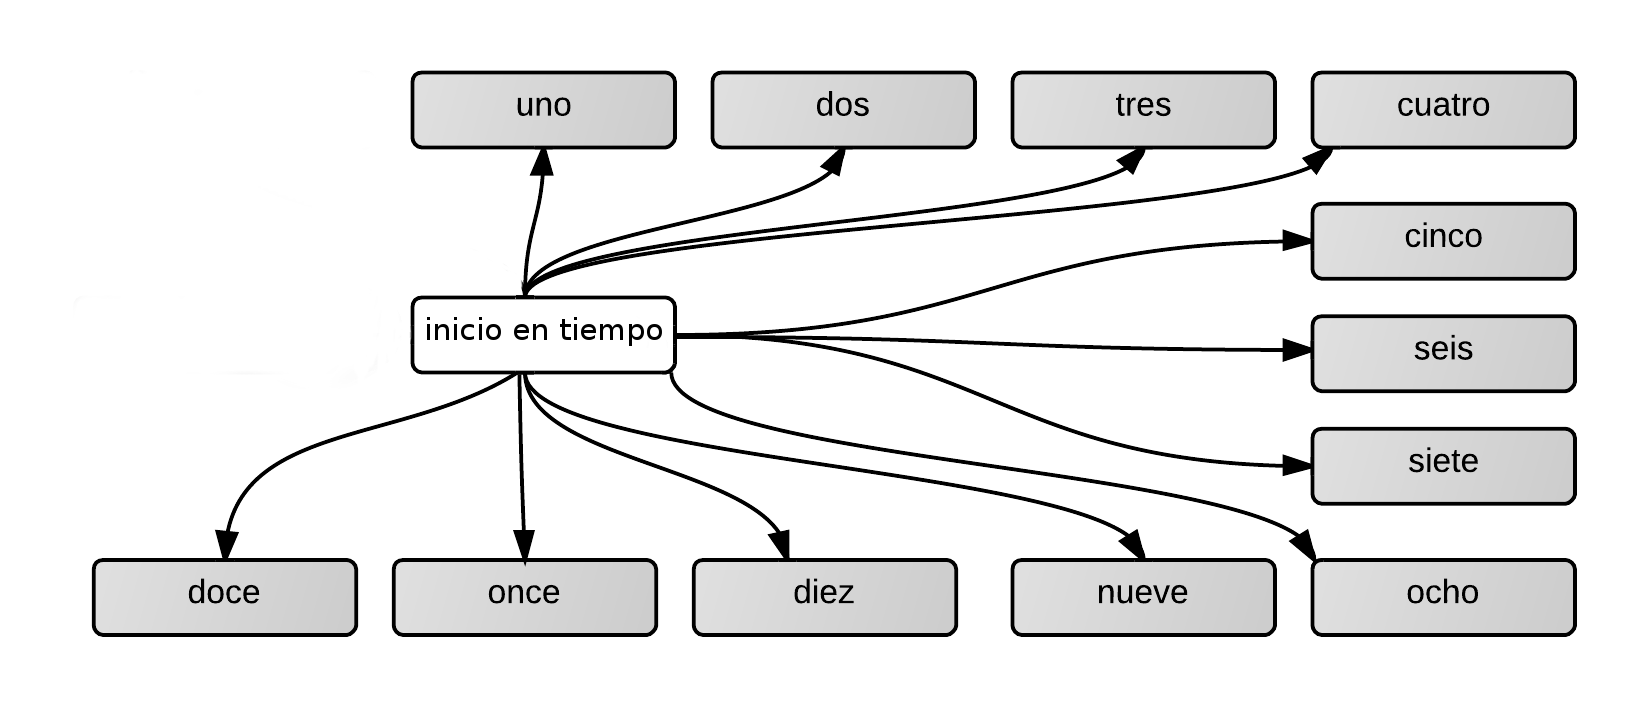
\includegraphics[width=1.1\linewidth]{./graphics/cmd-note-tiempo.png}
\caption{Comando que permite configurar el inicio de una nota dentro del comp\'as}
\label{figure:cmd-note-tiempo}
\end{minipage}
\end{figure}


\subsection{Diccionario}

Otro elemento requerido por \emph{Pocketsphinx} es el diccionario, que permite mapear
palabras a secuencia de fonemas. En la siguiente figura se muestra un fragmento del diccionario
utilizado por la aplicaci\'on.

\begin{figure}[H]
\begin{lstlisting}
REPRODUCIR RR E P R O D U S I R
PAUSAR P A U S A R
PARAR  P A R A R
GENERAR  J E N E R A R
PARTITURA P A R T I T U R A
SIGUIENTE S I G I E N T E
ANTERIOR A N T E R I O R
\end{lstlisting}
\caption{Fragmento del diccionario utilizad en \emph{Tamtam Listens}}
\end{figure}

La combinaci\'on de estos componentes es lo que permite a \emph{Pocketsphinx} realizar el
reconocimiento de los comandos de voz.

